\graphicspath{ {./figuresMeasure} }
\section{Measure}

\subsection{Conception}
Afin de valider nos simulation nous allons procéder aux mesures de quelques configurations choisies. 6 PCB seront fabriqué. Nous avons choisi de représenter un nombre de piste de 10 et 5. Car nos simulations de 20 pistes nous donnent une capacité beaucoup trop élevé. Pour chaque nombre de piste nous prenons deux rapport largeur et distance déjà simulé plus un plus faible pour étudier la possibilité de détecter de petite goutte. Le plan de cuivre du dessous est gardé pour tous. Pour les mesures, les cartes seront posées à plat et nous ne voulons pas être influencé par ce qui se trouve en dessous. Chaque PCB se verra attribué une lettre pour faciliter le nommage.

\begin{table}[!ht]
\begin{center}
\begin{tabular}[c]{lllll}
PCB & Nb piste & rapport larg/dist & Largeur de piste [mm] & distance entre piste [mm] \\
\hline
A & 10 & 2 & 4 & 2\\
B & 10 & 0.5 & 2 & 4\\
C & 10 & 0.22 & 1.1 & 4.9\\
D & 5 & 1 & 6 & 6\\
E & 5 & 0.5 & 4 & 8\\
F & 5 & 0.1 & 1.1 & 10.9
\end{tabular}
\caption{Liste des configurations sélectionné }
\end{center}
\end{table}

Le PCB est construit en suivant le plan mécanique de la figure \ref{plan}. Nous avons ajouté deux connecteurs SMB pour le relier à la carte de développement du convertisseur. Ils ont ensuite été pannelisé afin de les produire en une commande.

\begin{figure}[!ht]
\centering
 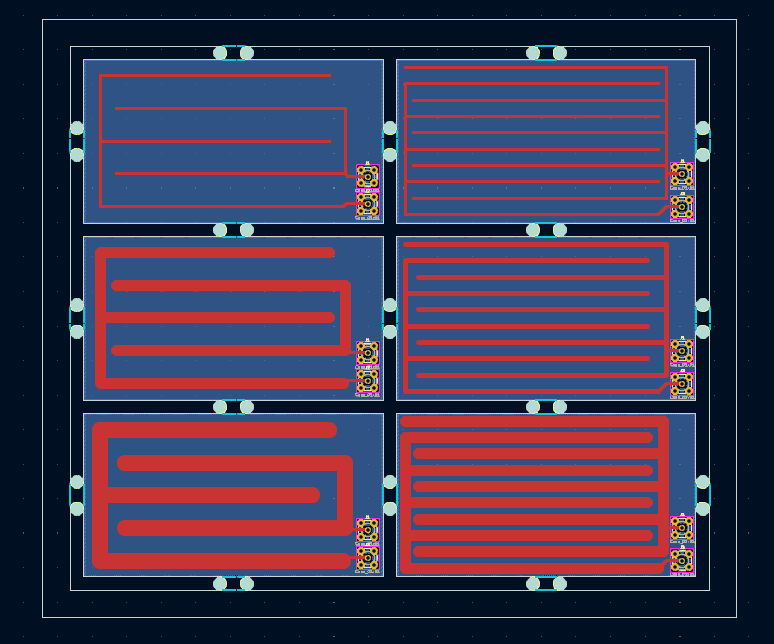
\includegraphics[width=12cm]{pannel.png}
 \caption{Pannel prêt à la production}
\end{figure}

\newpage

\subsection{Measure capacitive par filtre RC}

Avant de brancher nos cartes sur le convertisseur, nous allons effectuer une première mesure de la capacité afin de s'assurer d'être ou non à l'intérieur des bornes. Nous n'avons pas à notre disposition un analyseur d’impédance capable de mesurer de si faible capacité. Nous placerons la capacité à mesurer dans un filtre RC et déterminerons son temps de charge. Nous utiliserons un microcontrôleur pour générer un signal carré. Il faudra prendre en compte l’impédance et la capacité de la sonde d'oscilloscope car la résistance et la capacité mesurée se trouve dans le même ordre de grandeur.


\begin{figure}[!ht]
\centering
 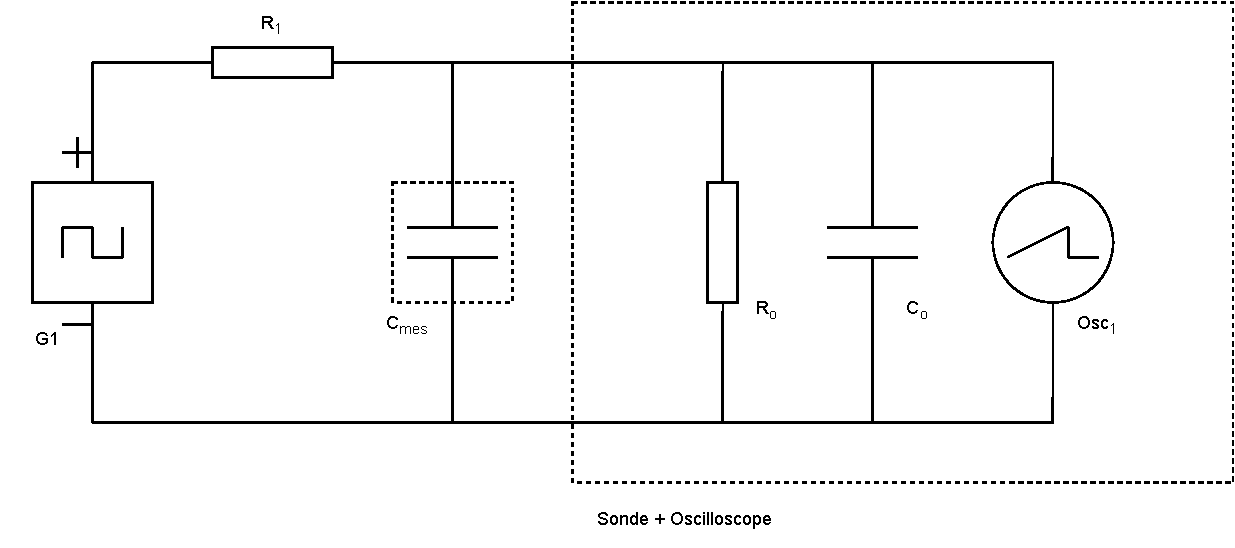
\includegraphics[width=10cm]{schemaMesure.pdf}
 \begin{description}
 \item[G1] Nucleo-L432KC, signal carré: 3.3V - 0V 10Hz
 \item[R1] 1 M$\Omega$
 \item[C$_{mes}$] PCB A,B,C,D,E,F
 \item[R$_o$] 10 M$\Omega$
 \item[C$_o$] à déterminer
 \item[Osc$_1$] Picoscope 6403D
\end{description}
 \caption{Schéma de mesure du filtre RC}
\end{figure}

L'impédance de la sonde et de l'oscilloscope est fourni mais la capacité est variable par la calibration de la sonde. Nous allons effectué une première mesure à vide sans $C_{mes}$ afin de déterminer $C_o$


\begin{figure}[!ht]
\centering
 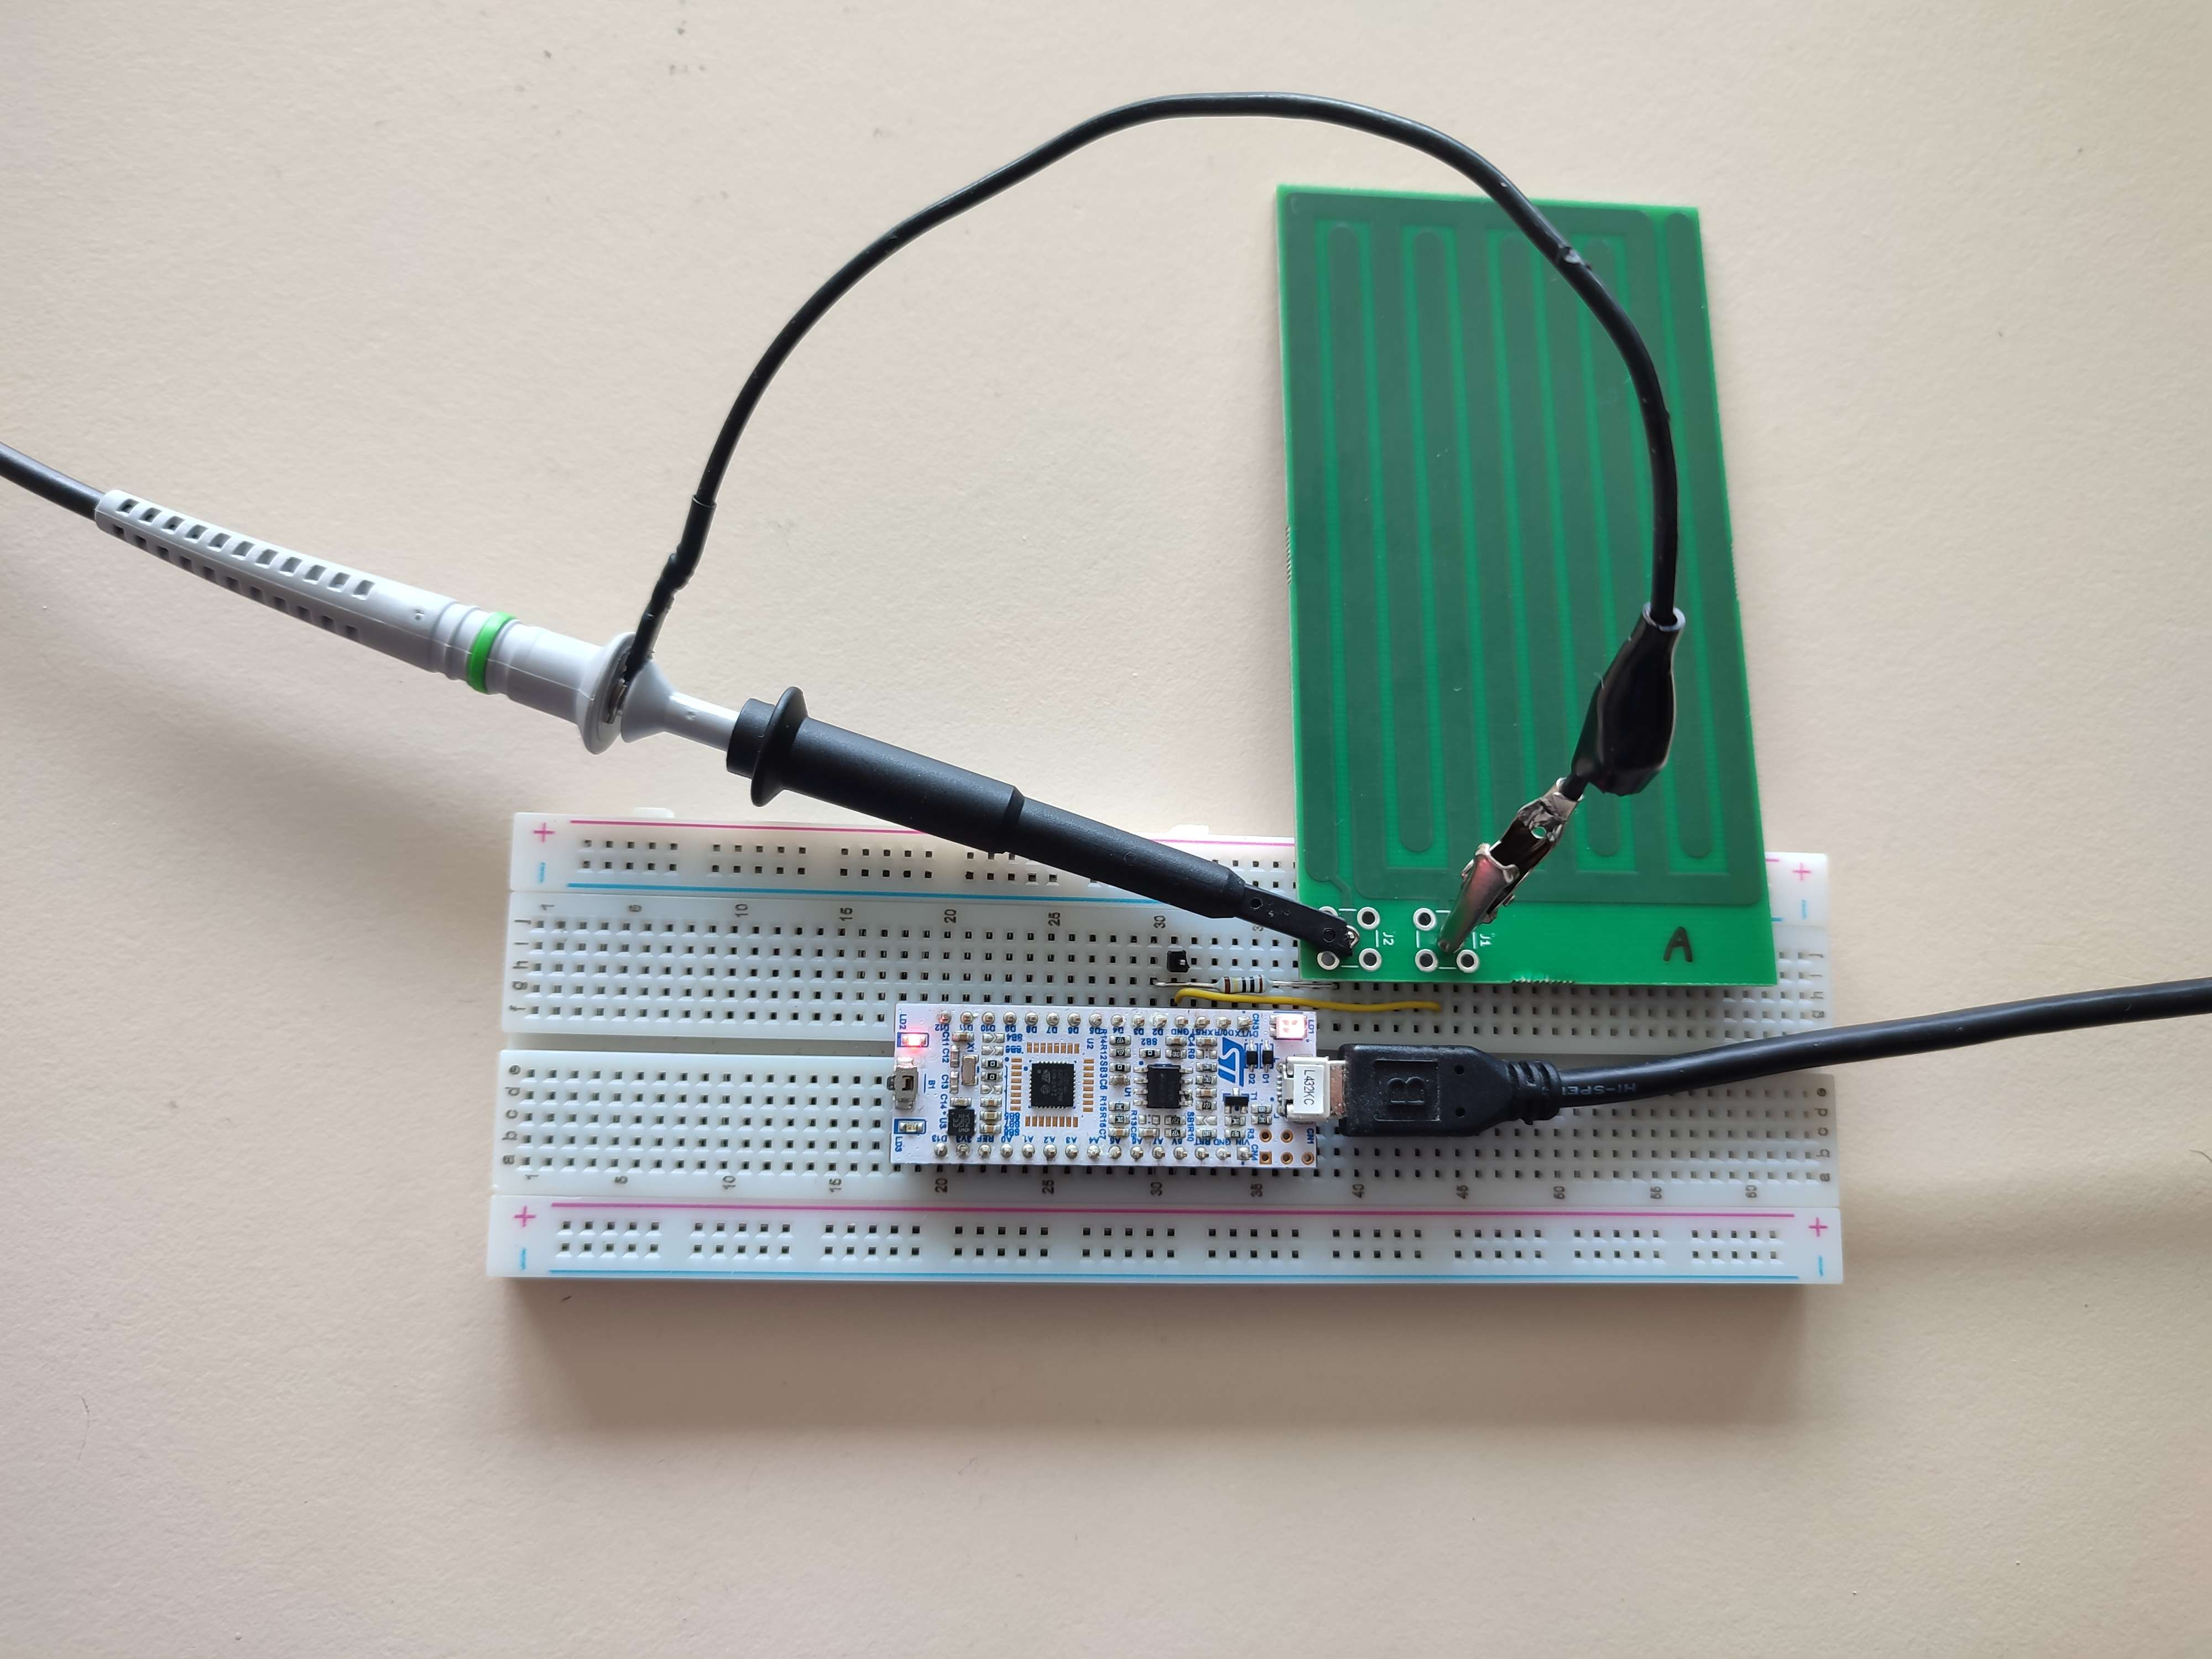
\includegraphics[width=10cm]{RCPhoto.jpg}
 \caption{Photo de la mesure RC}
\end{figure}

\newpage

Pour déterminer la constante de temps, nous utilisons le résultat de la résolution de l'équation différentiel d'un circuit RC: 

\begin{equation}
 U_{c}(t) = U_{in} \cdot (1 - e^{-\frac{t}{RC}})
\end{equation}
On pose $t = RC$
\begin{equation}
\frac{U_c(RC)}{U_{in}} = 1 - e^{-1} = 1 - 0.37 = 0.63
\end{equation}

 $U_c$ vaudra 63\% de $U_{in}$ 

 
Si on prend en compte la sonde et l'oscilloscope le circuit de mesure n'est pas un simple RC. Nous le simplifions par un schéma équivalent grâce à Thévenin. 
 
\begin{equation}
 R_{th} = R_1 // R_o = \frac{1}{\frac{1}{R_1} + \frac{1}{R_o}} = 909 [k\Omega]
\end{equation}

\begin{equation}
 U_{th} = U_{G1} * \frac{R_o}{R_1 + R_o} = 3 [V]
\end{equation}

Le schéma équivalent que nous utiliserons pour les calculs est le suivant:

\begin{figure}[!ht]
\centering
 \includegraphics[width=10cm]{schemaMesureTH.pdf}
 \begin{description}
 \item[R$_{th}$] 909$[k\Omega]$
 \item[U$_{th}$] 3[V]
\end{description}
 \caption{Schéma équivalent Thévenin de mesure du filtre RC}
\end{figure}

$C_{mes}$ et $C_o$ se combine. En laissant vide $C_{mes}$ nous pouvons déterminer $C_o$. Nous le soustrairons aux prochaines mesures pour déterminer $C_{mes}$.

\begin{figure}[!ht]
\centering
 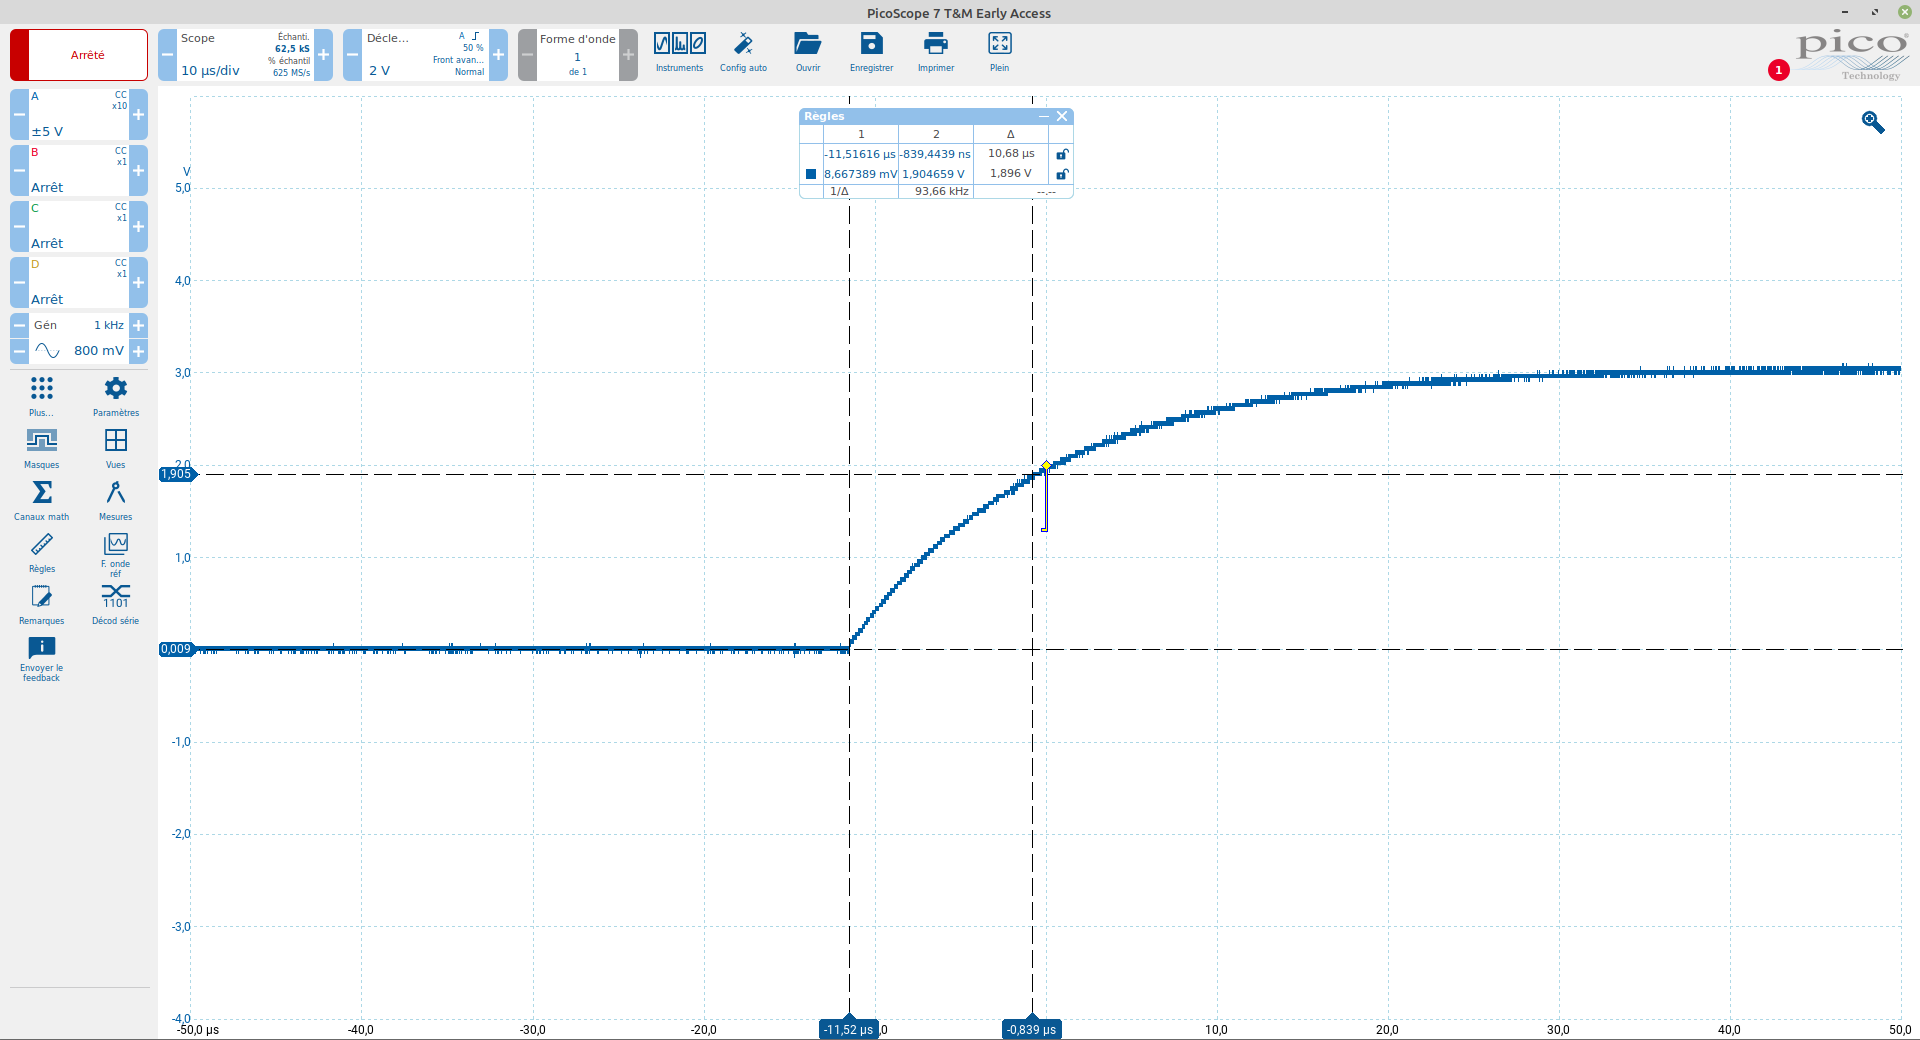
\includegraphics[width=14cm]{videe.png}
 \caption{Oscillogramme sans plaque}
\end{figure}

A 63\% de $U_{th}$ c'est à dire à 1.89 V nous observons un temps de \SI{10.68}{\micro\second} ce qui correspond à une capacité de $C_o = \frac{\tau}{R_{th}}= \SI{11.75}{\pico\farad}$. Nous pouvons à présent mesurer toutes nos cartes avec la même technique de mesure et en utilisant l'expression suivante:

\begin{equation}
 C_{mes} = \frac{\tau}{R_{th}} - C_o
\end{equation}

Nous comparons ces mesures à nos simulations lorsque cela est possible. 

\begin{table}[!ht]
\begin{center}
\begin{tabular}[c]{lll}
PCB & Mesure RC [pF] & Simulation [pF]\\
A & 47.3 & 47.4\\
B & 29.9 & 29.4\\
C & 23.2 & ×\\
D & 29.9 & 26.4\\
E & 23.2 & 19.9\\
F & 11.9 & ×
\end{tabular}
\caption{Résumé des mesures et de la simulation pour chaque carte (mesure complète: Annexe \ref{mesrc})}
\end{center}
\end{table}


Les mesures sont très proche de la simulation, on note une différence de moins de 2\% pour A et B ainsi que 10\% à 20\% pour D et E. Cette variation peut s'expliquer par plusieurs choses. D'une part la simulation prenait en compte une coupe de pistes droite alors que sur nos cartes des pistes supplémentaires sont présentes aux extrémités pour connecter les pistes. Le connecteur peut aussi ajouter une capacité non négligeable. De plus notre mesure n'est pas parfaite et nous avons simplifié l'effet que peut avoir la sonde et l'oscilloscope. Nous somme dans un ordre de grandeur avec de très faible courant. La mesure est facilement influençable par des grandeur parasite que nous négligeons habituellement. 

Ces mesures nous donnent une certaine confiance dans nos simulation. Nous pourrons en refaire de plus complexe dans une suite du projet tout en ayant une idée de comment les résultats se traduisent dans la réalité.  


\subsection{Convertisseur Capacitif}

Nous pouvons à présent essayer le convertisseur AD7150. Nous utiliserons sa carte de développement EVAL-AD7150. La carte est fourni avec un logiciel pour configurer et effectuer directement des mesures. Nous pouvons nous passer de microcontrôleur pour l'instant.

Nous allons commencer par mesurer la carte F. C'est la seule qui rentre dans les borne du convertisseur et pourra être mesuré directement. 

\begin{figure}[!ht]
\centering
 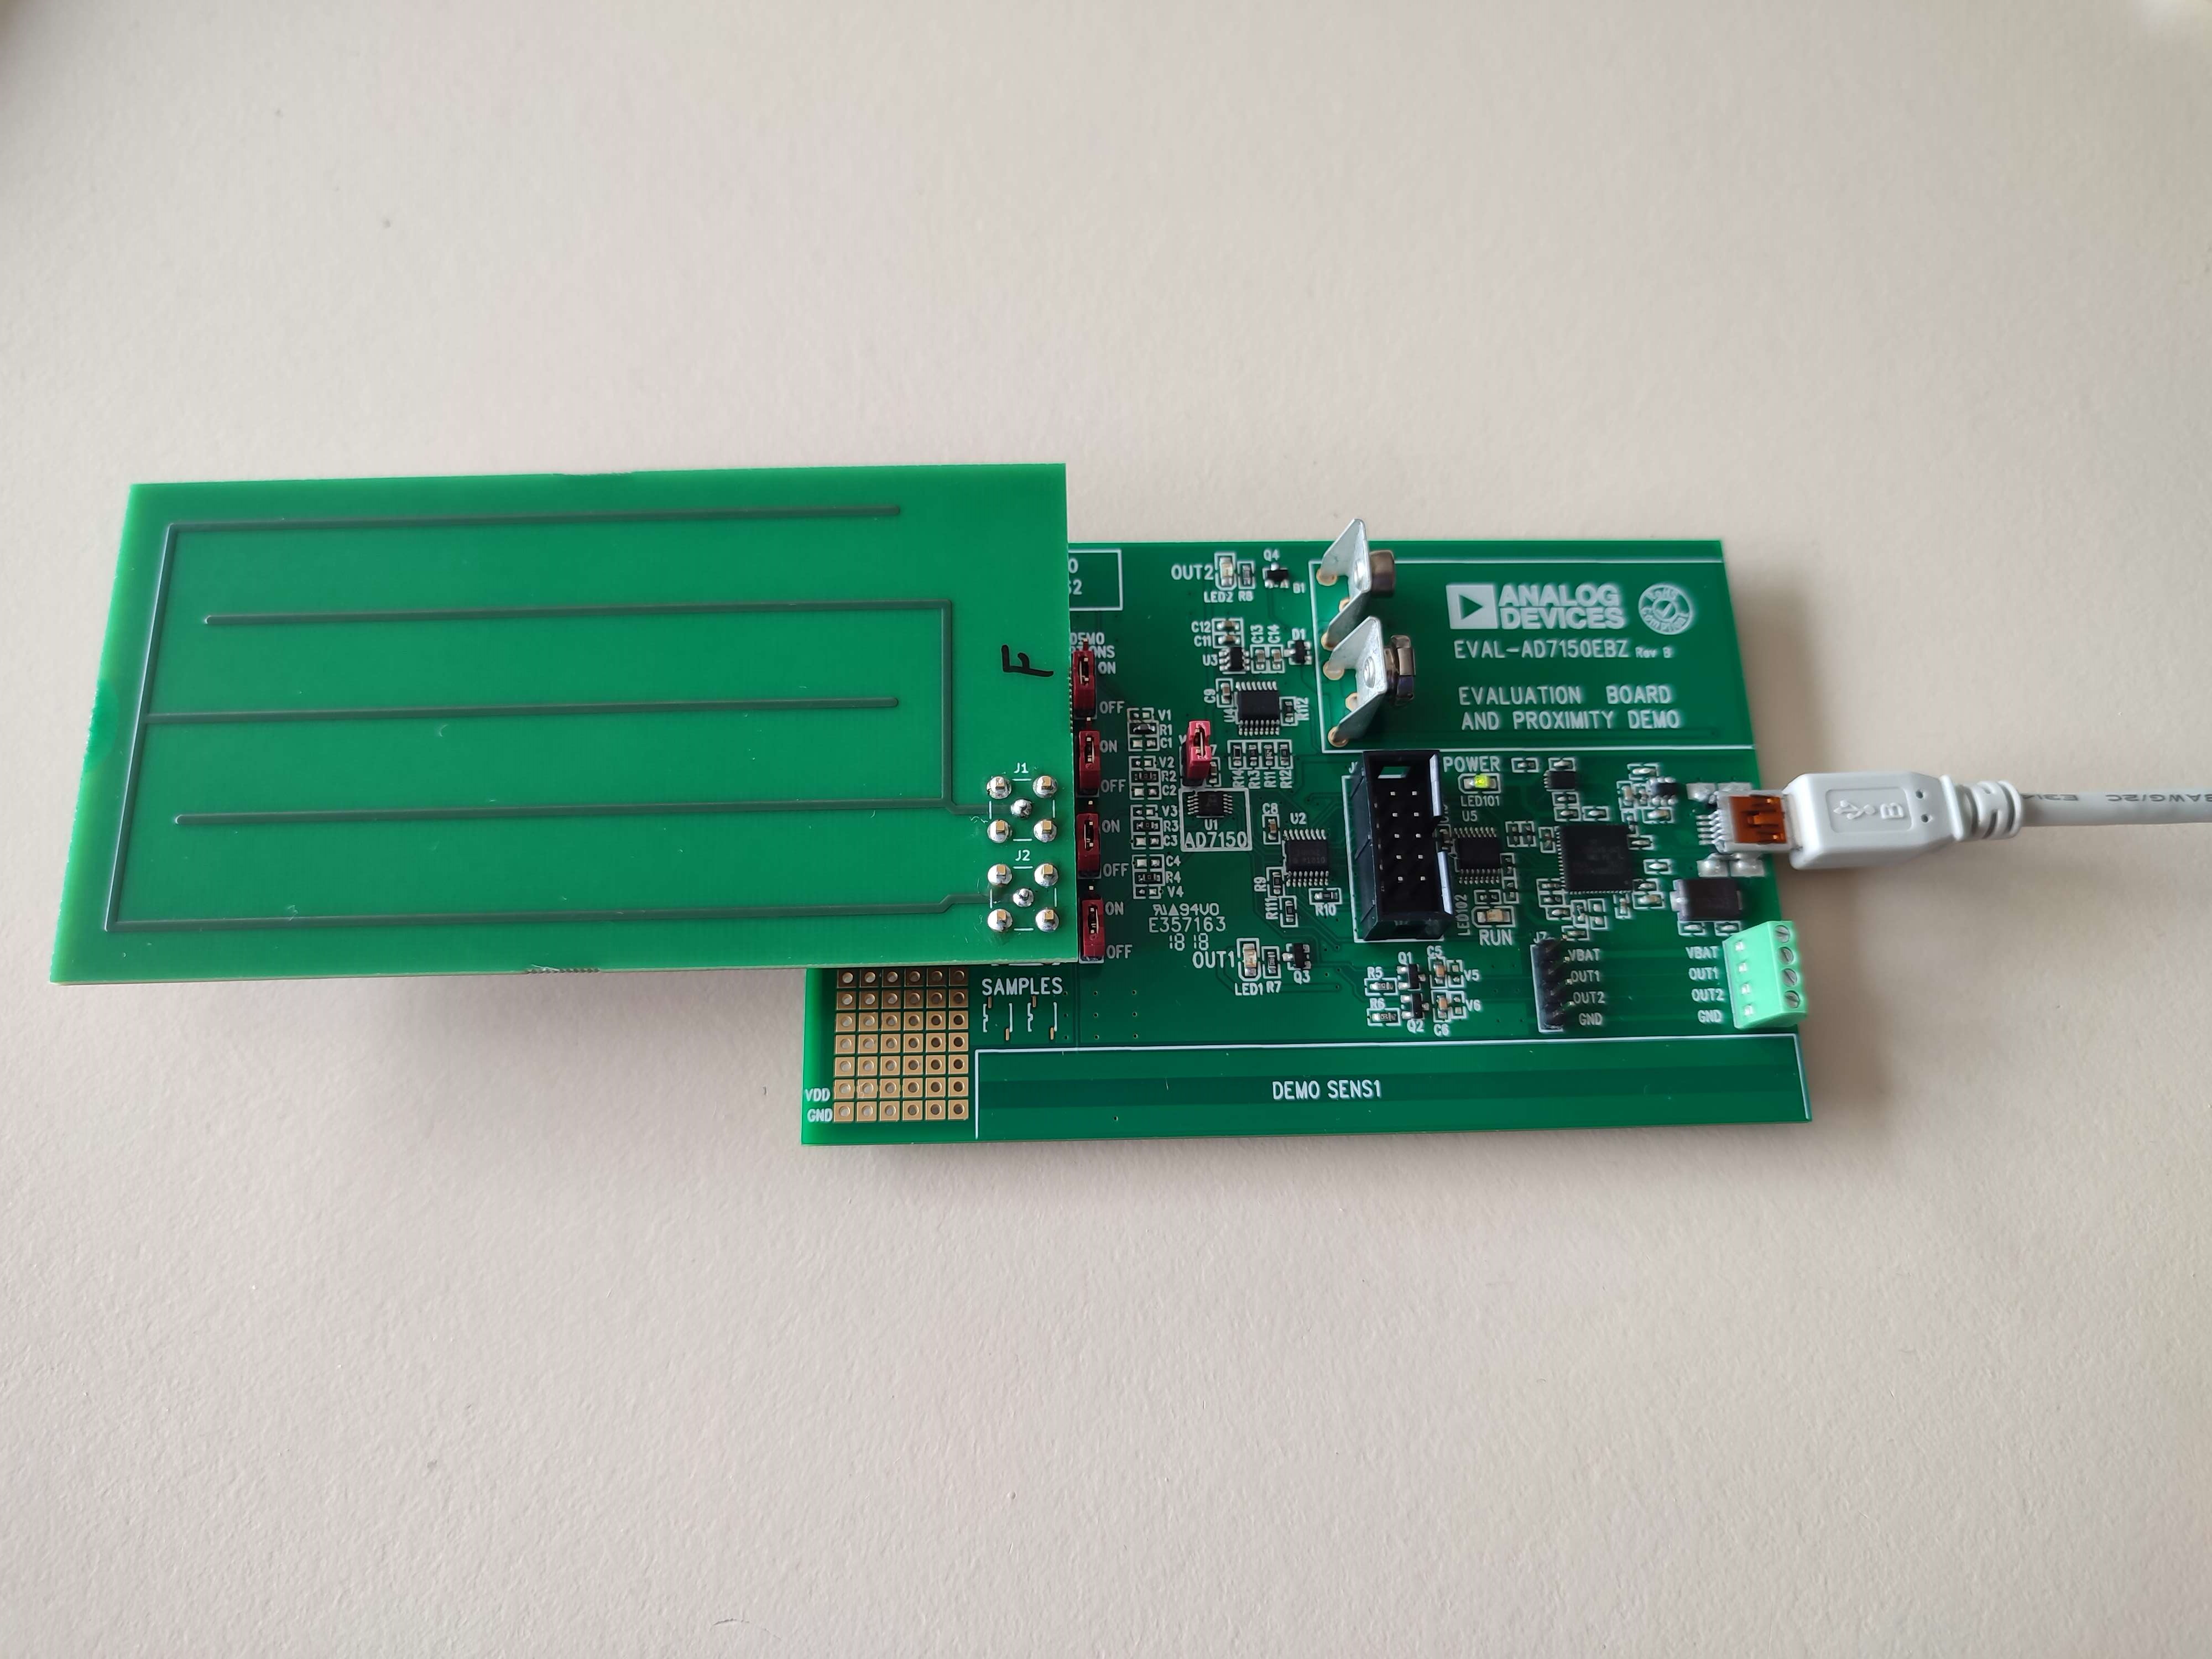
\includegraphics[width=10cm]{ADPhoto.jpg}
 \caption{Photo de la mesure de F avec EVAL-AD7150}
\end{figure}

\newpage

Pour cette première mesure le convertisseur est configuré avec une sensibilité de 2pF. Le CapDAC qui est l'offset est trouvé en le modifiant jusqu'à ce que la mesure ne sature plus. 

\begin{figure}[!ht]
\centering
 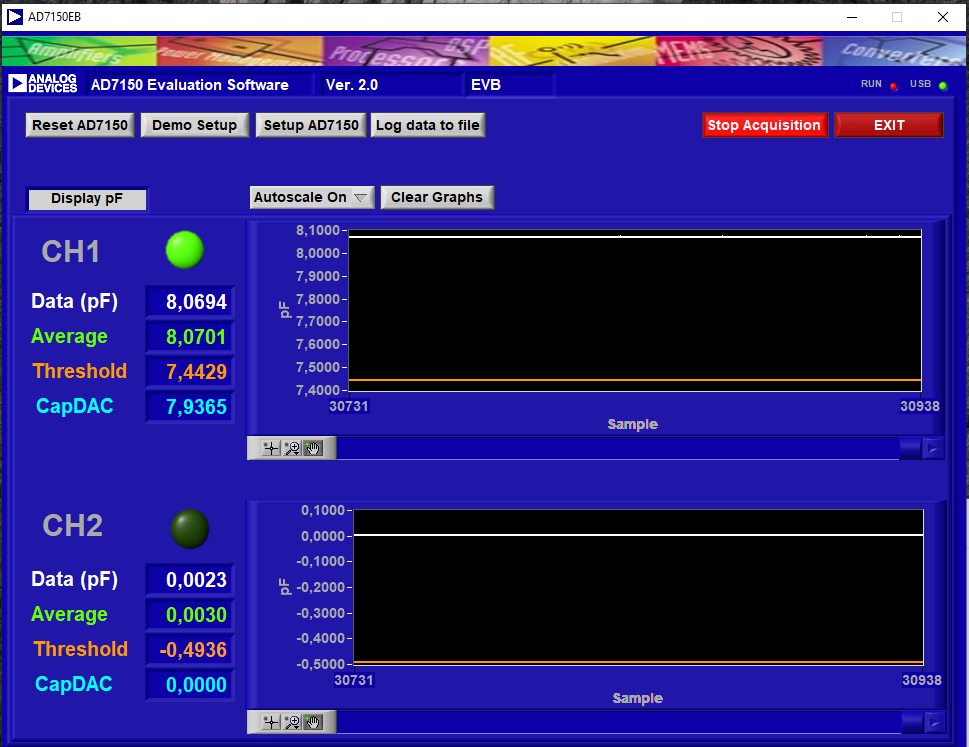
\includegraphics[width=10cm]{Fadair.png}
 \caption{Mesure de la carte F avec l'interface de la carte de développement de l'AD7150  }
\end{figure}

Nous mesurons une capacité de 8.1 pF pour 11.9 pF mesuré par RC. Cette différence s'explique d'une part par la précision d'une mesure RC expliqué précédemment et d'une autre par problème propre au convertisseur AD7150. 

Nous avons remarqué, lors de nos mesures, que lorsque nous approchons la main de la carte la capacité mesuré diminue fortement, ce qui ne se produisait pas avec le filtre RC. Cela viens de l’influence de la capacité parasite à la masse. Aucuns des deux pôle de la carte ne sont reliés à la masse. Si une capacité apparaît entre un des pôle et la masse des charges seront perdues et ne seront pas mesurées par le convertisseur ce qui diminuera la capacité observée. Même si nous somme éloigné, du capteur une capacité parasite est présente en partie à cause du plan de masse de la carte de développement. Nous ne pourrons malheureusement pas mesurer correctement la capacité absolue de nos cartes. 

Nous pouvons cependant commencer à détecter à titre indicatif des gouttes d'eau. 

\begin{figure}[!ht]
\centering
 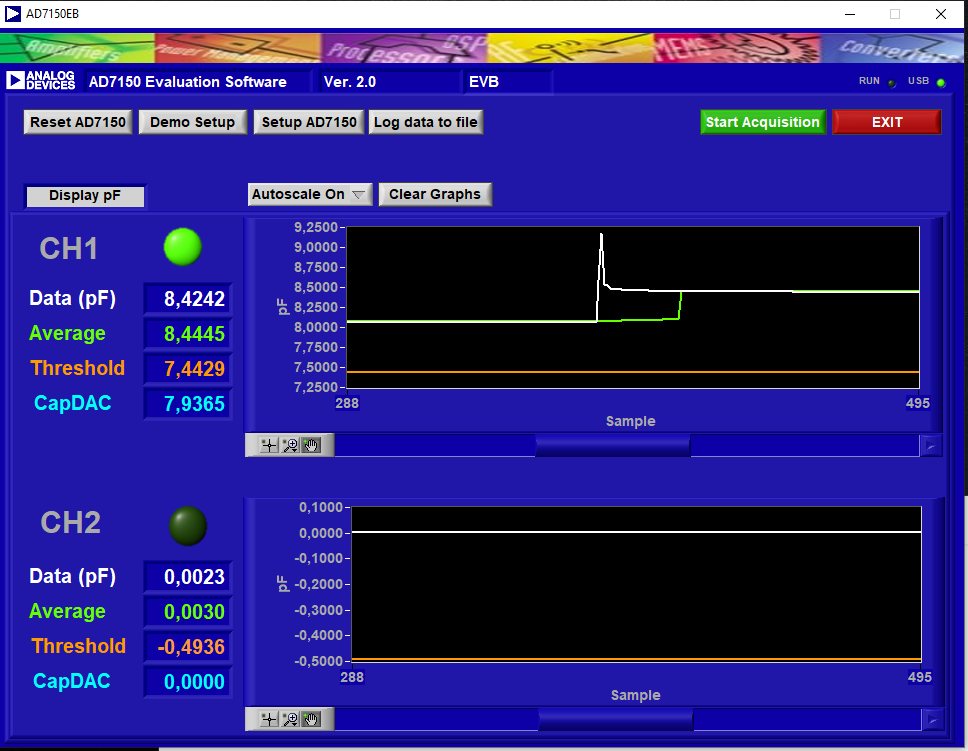
\includegraphics[width=10cm]{fadeau.png}
 \caption{Mesure de la carte F en faisant tomber une goutte d'eau}
\end{figure}

\newpage
Ces mesures ne permettent pas de sortir des chiffre précis, mais nous introduit le comportement de l'eau sur notre capteur. Pour pouvoir essayer les autres cartes, malgré qu'elles soient hors borne, nous avons mis une capacité de 10pF en série avec notre dipôle. Sur la carte de développement nous remplaçons par notre capacité une résistance de 0 ohm qui fait le pont entre le convertisseur et le connecteur. La capacité parasite de masse est trop compliqué à calculer dans cette configuration. Nous ne prendrons pas en compte la valeur absolue de la mesure mais seulement l’influence de l'eau. Il apparaît clairement qu'avec des pistes plus serrées, les gouttes sont plus facilement détectées malgré la perte de sensibilité dû à l'ajout d'une capacité en série. 
La taille et la position de la goutte influence beaucoup la détection de celle-ci. Un travail supplémentaire devra être effectué pour optimiser le peigne. La simulation en 2 dimension ne suffira pas pour représenter la géométrie et le placement d'une goutte d'eau.

